\chapter[Pre-Execution Prevention of Privacy-Route Misalignment]{Pre-Execution Prevention of Privacy-Route Misalignment: Evidence-Sealed Registration}
\label{ch:evidence-sealed-registration}

\section{From Diagnosis to Prevention}
\label{sec:ch3-diagnosis-to-prevention}

Chapter~\ref{ch:post-execution-validation} treated a completed execution as a
frozen object.  Its validator reopened the available evidence, compared that
evidence with a requested privacy sentence, and released only wording supported by
the registered transformation and accounting premises.  That decision is useful
after training, but it has a temporal limit: it cannot undo an execution whose
sampler, adjacency, accountant, or data transformation was already configured
under incompatible assumptions.  Once such a route has run, a fail-closed report
can suppress an unsupported claim, but it cannot convert the execution into the
route that the claim would have required.

This chapter therefore moves the \AuditablePrivacy{} axis from post-execution
diagnosis to pre-execution prevention.  The object is an owner-sampled
differentially private stochastic gradient descent (DP-SGD) route installed behind
one extensible training interface.  A route label is meaningful only when it
jointly identifies the neighboring relation, owner sampler, sensitivity and noise
geometry, accountant, executor, data transformation, and evidence obligations.
Individually valid components do not automatically form a valid composition.  For
example, a Bernoulli sampler analyzed under add/remove adjacency and a fixed-size
sampler analyzed under replace-one adjacency may each be legitimate.  Substituting
the second sampler into a handler that retains the first route's sensitivity and
accountant, however, does not preserve either registered statement.

The practical risk is subtle because training can still complete.  A strict
contract may contain values of the right primitive types, the selected objects may
all be callable, and a downstream metric may appear reasonable.  Those checks do
not show that the installed handler represents one coherent privacy route.
Implementation studies have demonstrated that sampling and accounting
misalignment can materially change the privacy behavior of DP-SGD
systems~\cite{chua2024implementations}.  Implementation and auditing guidance
accordingly requires the privacy unit, neighboring relation, sampling rule,
clipping convention, and accountant to be reviewed as one mechanism
description~\cite{kifer2020guidelines,ponomareva2023dpify,near2025guidelines}.

The question addressed here is consequently narrower than general program
verification but stronger than field-by-field validation:

\begin{quote}
What must pre-execution route registration bind so that a mixture of components
from two registered owner-DP-SGD routes cannot retain either route label?
\end{quote}

The proposed answer is \emph{route-label registration consistency}.  Each
registered implementation, called a handler, owns an exact nominal route and a
complete core containing its types, route-local objects, source-resolved callables,
and seven required obligations.  A passing evidence report commits to that core.
Before a serialized contract may be dispatched, registration recomputes the core
from live objects and requires exact identity, schema, report, and digest
agreement.  Only then does a branch-free generic dispatcher invoke the selected
handler's parser and compiler.

This construction establishes a pre-execution label boundary.  If a prespecified
hybrid handler fails the predicate, the conclusion is only that it cannot retain
either registered endpoint label.  The rejection does not prove that the hybrid
is nonprivate, and acceptance does not prove that arbitrary code faithfully
implements differential privacy.  The distinction matters because the scientific
contribution is the joint predicate and its counterfactual evaluation, not the use
of SHA-256 or the existence of a wrapper around a single route.

The contributions of this chapter are summarized as follows.

\begin{itemize}
    \item It defines route-label registration consistency for owner-sampled
    DP-SGD.  One route identity jointly binds adjacency, sampler, sum sensitivity,
    Gaussian scale, accountant, executor, transformation, and the evidence chain
    needed to support that identity.

    \item It realizes the criterion as an evidence-sealed registration judgment.
    A handler registers exact contract and plan types, strict parser and compiler
    callables, a route-local registry, and seven source-resolved obligations.
    Generic exact-key dispatch rechecks this joint core before compilation and
    execution.

    \item It separates handler installation from contract and lifecycle checks.
    The evaluation compares contract-only and full-lifecycle boundaries, then
    measures weak, source-bound, and complete-core registration over a fixed
    handler-splice lattice.

    \item It tests bounded extension across three established routes.  These are
    Bernoulli sampling with add/remove adjacency (\RouteP), fixed-size sampling
    with replace-one adjacency (\RouteF), and per-epoch random allocation with
    add/remove adjacency (\RouteA).  The experiment checks exact preservation of
    old objects, controlled route separation, and accountant--execution
    correspondence.
\end{itemize}

The phase boundary is strict.  This chapter introduces no new sampler,
amplification theorem, accountant, owner-level DP mechanism, general DP compiler,
privacy type system, or execution-attestation protocol.  It performs no
post-execution privacy-unit conversion.  The three route mechanisms and their
privacy analyses are prior work; the object studied here is the finite
registration boundary through which those heterogeneous routes are installed and
executed.  Its guarantees are conditional on honest source, executor, evidence
construction, and verification, a limitation made explicit in
Section~\ref{subsec:ch3-conditional-scope}.

\section{Background and Problem Setting}
\label{sec:ch3-background}

\subsection{Owner-Sampled DP-SGD Routes}
\label{subsec:ch3-owner-routes}

Let the protected training dataset be
\(\mathcal D=(\mathcal D_u)_{u\in\mathcal U}\), where
\(\mathcal D_u\) is the collection attributed to one person, patient, subject,
device, or sequence \(u\).  Preparation produces generated records \(w\) and an
attribution map \(\alpha(w)\).  Every route registered in this chapter requires
\(\alpha(w)=\{u\}\): each generated record has exactly one owner.  A record
attributed to multiple owners changes the neighboring relation and sensitivity
analysis and is therefore rejected rather than silently assigned to one of the
three routes~\cite{ganesh2025multiuser}.

The contribution policy is fixed before protected training and operates
owner-locally.  Under public caps, it may retain or select records inside
\(\mathcal D_u\), but one owner's contribution vector may not depend on another
owner's raw data.  The preprocessing transform is likewise fixed as public side
information.  It is not fitted on protected input inside the executor.  These
conditions keep the registered owner unit, mapping, and contribution rule stable
across neighboring datasets; they are assumptions of the route statement rather
than properties established by a digest.

For a participating owner \(u\) at step \(s\), the executor applies the
owner-local policy, computes a mean-loss gradient \(g_{u,s}\), and clips that
vector to threshold \(C\).  Let \(\theta_s\) be the model parameters,
\(\mathcal B_s\) the participating-owner set, \(\eta\) the learning rate,
\(\sigma\) the noise multiplier, and \(D_{\mathrm{norm}}\) a public normalization
constant.  Every route uses the common update

\begin{equation}
\begin{aligned}
    \bar g_{u,s}
        &=
        g_{u,s}
        \min\!\left\{1,\frac{C}{\lVert g_{u,s}\rVert_2}\right\},\\
    Z_s
        &\sim
        \mathcal N\!\left(0,\sigma^2 C^2 I\right),\\
    \theta_{s+1}
        &=
        \theta_s
        -
        \frac{\eta}{D_{\mathrm{norm}}}
        \left(
            \sum_{u\in\mathcal B_s}\bar g_{u,s}+Z_s
        \right),
        \qquad
        0\leq s<\TrainingSteps .
\end{aligned}
\label{eq:ch3-common-update}
\end{equation}

The denominator \(D_{\mathrm{norm}}\), denoted \(D\) in the source research
profiles, is fixed post-processing; it is never replaced by the realized number of
owners in \(\mathcal B_s\).  The common arithmetic does not erase the differences
among routes.  Their sampling laws, neighboring relations, sensitivities, and
accountants remain distinct.

\paragraph{Route \RouteP: Bernoulli/add-remove.}
The public plan fixes \(\SamplingRate\), \(\TrainingSteps\), \(C\), \(\sigma\),
and \(D_{\mathrm{norm}}\).  At every step, each present owner is included
independently with probability \(\SamplingRate\).  Adding or removing one owner
changes the clipped sum by at most \(C\).  When
\(\mathcal B_s=\varnothing\), the aggregate contribution is zero, but Gaussian
noise is still sampled and the optimizer advances.  The route uses an
add/remove-adjacency accountant based on repeated subsampling and R{\'e}nyi
differential privacy (RDP) composition
~\cite{mironov2017renyi,wang2019subsampled,yousefpour2021opacus}.

\paragraph{Route \RouteF: fixed-size/replace-one.}
The public plan fixes a population of \(\OwnerPopulation\) owner positions and
\(m,\TrainingSteps,C,\sigma,D_{\mathrm{norm}}\), with
\(D_{\mathrm{norm}}=m>0\).  At every step, simple random sampling without
replacement draws a uniformly random subset of exactly \(m\) distinct positions.
Replacing one owner can replace one clipped vector by another, so the sum
sensitivity is bounded by
\(\lVert\bar g-\bar g'\rVert_2\leq2C\).  Noise with standard deviation
\(\sigma C\) consequently corresponds to normalized noise \(\sigma/2\) for the
registered fixed-size replace-one accountant.  Route \RouteF{} does not inherit
Route \RouteP's adjacency or accountant merely because both execute
Equation~\eqref{eq:ch3-common-update}; its sampling analysis follows the
fixed-size literature~\cite{wang2019subsampled,birrell2024fixed}.

\paragraph{Route \RouteA: random-allocation/add-remove.}
For each of \(\EpochCount\) epochs, every owner independently draws a uniformly
random \(\AllocationCount\)-subset of \(t\) candidate steps and participates at
exactly those steps.  The total schedule is
\(\TrainingSteps=\EpochCount t\).  One owner's participation is therefore coupled
across steps, unlike Route \RouteP, while the number of active owners at one step
is not fixed, unlike Route \RouteF.  The sum has add/remove sensitivity \(C\), and
every scheduled step adds noise and advances the optimizer, including an empty
step.  This route uses the established random-allocation or balanced-iteration
participation law and a conservative direct bound; tighter privacy-loss
distribution accounting remains prior work
~\cite{shenfeld2025randomallocation,feldman2026pld,dong2026optimal}.

The public-plan invariants differ accordingly.  Route \RouteP{} fixes
\(\SamplingRate\), \(\TrainingSteps\), and \(D_{\mathrm{norm}}\); none derives
from the observed retained-owner count.  Route \RouteF{} fixes
\(\OwnerPopulation\), \(m\), \(\TrainingSteps\), and \(D_{\mathrm{norm}}\) for
a replace-one domain rather than using observed batch statistics.  Route
\RouteA{} makes \(t\), \(\AllocationCount\), \(\EpochCount\), and
\(D_{\mathrm{norm}}\) public, while assignments and realized participation remain
private.  The benchmark profiles used later are exact public fixtures.
This restriction prevents private, data-dependent schedule facts from entering a
supposedly invariant plan, but it also limits the release claim as discussed in
Section~\ref{subsec:ch3-conditional-scope}.

\subsection{Route-Label Misalignment}
\label{subsec:ch3-route-label-misalignment}

A route is not a sampler name or an accountant identifier.  The dissertation
represents its nominal identity as

\begin{equation}
    \RouteIdentity
    =
    \left(
        {\sim}_{\rho},
        \mathsf S_{\rho},
        \Delta_{\rho},
        \nu_{\rho},
        \mathsf A_{\rho},
        \mathsf X_{\rho}
    \right),
\label{eq:ch3-route-identity}
\end{equation}

The six entries are adjacency, owner sampler, sum sensitivity, Gaussian scale,
accountant, and executor.  The mapping, owner-local policy, preprocessor, and
artifact chain are bound around this nominal core.  A serialized contract is
route-label misaligned when it or its installed handler combines fields that do
not jointly instantiate one registered \(\RouteIdentity\), even if each field
could be valid in a different endpoint.

Table~\ref{tab:ch3-contract-surface} summarizes the shared structural surface.
Each row is instantiated nominally by one route.  An unsupported value or a
mixture across registered routes must produce a named rejection rather than a
fallback interpretation.

\begin{table}[tbp]
    \centering
    \caption{Route-specific registration contract surface}
    \label{tab:ch3-contract-surface}
    \small
    \setlength{\tabcolsep}{4pt}
    \renewcommand{\arraystretch}{1.16}
    \begin{tabular}{@{}
        >{\raggedright\arraybackslash}p{0.17\textwidth}
        >{\raggedright\arraybackslash}p{0.73\textwidth}@{}}
        \toprule
        \textbf{Layer} & \textbf{Required binding or rejection} \\
        \midrule
        Privacy &
        Owner unit; exact adjacency; fixed \((\varepsilon,\delta)\) \\

        Mechanism &
        Sampler; \(\SamplingRate\), \((\OwnerPopulation,m)\), or
        \((t,\AllocationCount,\EpochCount)\);
        \(\TrainingSteps,C,\sigma,D_{\mathrm{norm}}\); sensitivity;
        empty-step rule \\

        Data &
        Single attribution; owner-local policy; exact mapping;
        public-fixed transformation \\

        Program &
        Model, loss, optimizer, route executor, accountant, and source bundle \\

        Artifacts &
        Typed public-plan digest; private mapping binding; model--run--summary--
        collection links \\
        \bottomrule
    \end{tabular}
\end{table}

Strict parsing of Table~\ref{tab:ch3-contract-surface} is necessary but
insufficient.  A contract can be exact while the handler selected by its route
identifier contains a parser from one endpoint, an accountant from another, and
source witnesses that remain individually well formed.  Conversely, a handler can
be coherent while a later mapping, preprocessor, executor, or serializer breaks
the lifecycle relation.  The design therefore separates three boundaries:
handler registration, exact contract compilation, and execution/artifact
verification.

A reproduced historical case illustrates the label problem.  The training loader
used an epoch shuffle with a drop-last rule, while the accounting description used
a per-step fixed-population hypergeometric model.  No exact law correspondence
between those two objects had been established.  The correct registration outcome
is therefore that the exact accounting label is unsupported.  This classification
does not establish that the alternative execution violated privacy; it prevents an
unproved route interpretation from being released under an existing label.

Several adjacent research areas address different objects.  Established work
supplies RDP composition and privacy analyses for fixed-size sampling, random
allocation, and user-level grouping
~\cite{mironov2017renyi,wang2019subsampled,birrell2024fixed,
shenfeld2025randomallocation,chua2024mind}.  This chapter treats those analyses as
heterogeneous registered endpoints and claims no accounting novelty.

Formal and typed DP systems can prove or refute semantic privacy properties, and
frameworks such as OpenDP provide explicit domains, metrics, and stability or
privacy maps~\cite{near2019duet,wang2020checkdp,hay2020opendp}.  Testing systems can
seek counterexamples or empirically audit an implementation
~\cite{kong2024auditorium,chua2024implementations}.  The present object is more
restricted: it checks one finite, author-constructed installation boundary and
measures rejection and preservation without claiming a refinement proof or an
arbitrary-input privacy test.

Software provenance and reproducible builds address a different layer.  in-toto
binds signed layouts and artifact flow, while reproducible-build methods seek
bit-identical reconstruction~\cite{torresarias2019intoto,lamb2022reproducible}.
Either could strengthen the evidence chain used here, but neither alone specifies
that an adjacency, sampler, sensitivity, accountant, and executor constitute one
DP route.  Verifiable and confidential DP systems further address authenticated or
cryptographic evidence of computation~\cite{narayan2015verifiable,
shamsabadi2024confidential}.  The registration seal below assumes honest checked
components and must not be interpreted as such attestation.

\section{Evidence-Sealed Route Registration}
\label{sec:ch3-registration}

\subsection{Registered Routes and Complete-Core Seal}
\label{subsec:ch3-complete-core}

Let a handler \(\RouteHandler\) contain an exact route identifier and schema
identifier, the nominal tuple \(\RouteIdentity\) from
Equation~\eqref{eq:ch3-route-identity}, an exact contract type
\(\tau_{\mathrm{ctr}}\), an exact public-plan type \(\tau_P\), a strict parser
\(p\), a compiler \(c\), a route-local registry object \(r_h\), and a witness map
\(W\).  The \emph{complete handler core} is the canonical serialization

\begin{equation}
    \RouteCore{\RouteHandler}
    =
    \operatorname{canon}\!\left(
        \mathrm{id},
        \mathrm{schema},
        \RouteIdentity,
        \tau_{\mathrm{ctr}},
        \tau_P,
        p,
        c,
        r_h,
        W
    \right).
\label{eq:ch3-complete-core}
\end{equation}

Canonicalization fixes field order, type representation, callable identity, source
path representation, and serialization before hashing.  It prevents two
semantically different field structures from being accepted merely because an
ordinary map happens to produce the same presentation order.  The handler's route
and schema identifiers are included inside the core rather than treated only as
lookup keys.

The witness map has exactly seven distinct obligation keys:

\begin{equation}
\begin{split}
    \mathcal O
    =\{&
        \textsf{strict\_parser},
        \textsf{strict\_compiler},
        \textsf{accountant},
        \textsf{numeric\_crosscheck},\\
      & \textsf{executor},
        \textsf{postcompile\_integrity},
        \textsf{source\_binding}
    \}.
\end{split}
\label{eq:ch3-obligation-set}
\end{equation}

Every witness names the exact callable, its resolved repository path, and its file
digest.  The keys are not interchangeable aliases: the accountant and numerical
cross-check, for example, must be separate obligations even when they reside in
the same source file.  The route-local registry must expose nominal fields that
agree with \(\RouteIdentity\), and the executor witness must identify an executor
that has passed the route's registration checks.

The route evidence report \(\RouteEvidence\) is constructed before protected
execution.  Its own path and digest remain outside
\(\RouteCore{\RouteHandler}\) to avoid a circular commitment in which the core
would contain the digest of a report that contains the core.  Those values are
bound separately.  Writing \(\operatorname{SHA256}\) for the deterministic
commitment, registration accepts only if

\begin{equation}
\begin{aligned}
    \RouteEvidence \vdash \RouteHandler\ \textsf{registered}
    \quad\Longleftrightarrow\quad&
    \operatorname{dom}(W)=\mathcal O,\\
    &\operatorname{Consistent}(\RouteHandler,W),\\
    &\RouteEvidence.\mathrm{status}=\textsf{PASS},\\
    &\RouteEvidence.\mathrm{id}=\RouteHandler.\mathrm{id},\\
    &\RouteEvidence.\mathrm{schema}=\RouteHandler.\mathrm{schema},\\
    &\operatorname{SHA256}(\RouteEvidence.\mathrm{core})
      =\RouteEvidence.\mathrm{core\_hash}\\
    &\hspace{29mm}
      =\operatorname{SHA256}\!\left(\RouteCore{\RouteHandler}\right).
\end{aligned}
\label{eq:ch3-registration-judgment}
\end{equation}

Registration requires more than the digest equalities in
Equation~\eqref{eq:ch3-registration-judgment}.  The checker also matches the
separately declared report digest and report-payload digest.  Every live file must
equal its report entry, and every callable must resolve to the declared source.
The parser, compiler, executor, and integrity method require exact witnesses,
obligation keys must be distinct, and the route-local registry must agree with the
handler's nominal fields.  A missing, duplicate, renamed, or aliased obligation
causes registration to fail.

The resulting decision is a machine-checked conformance predicate.  SHA-256
supplies only deterministic commitment to declared artifacts.  It does not prove
the privacy theorem referenced by the accountant, the semantics of arbitrary
source code, faithful runtime execution, or the quality of random coins.  The
central test is whether the complete jointly registered object remains one of the
installed endpoints when its fields are subjected to the controlled
counterfactuals in Section~\ref{subsec:ch3-lifecycle-ablation}.

\begin{figure}[tbp]
    \centering
    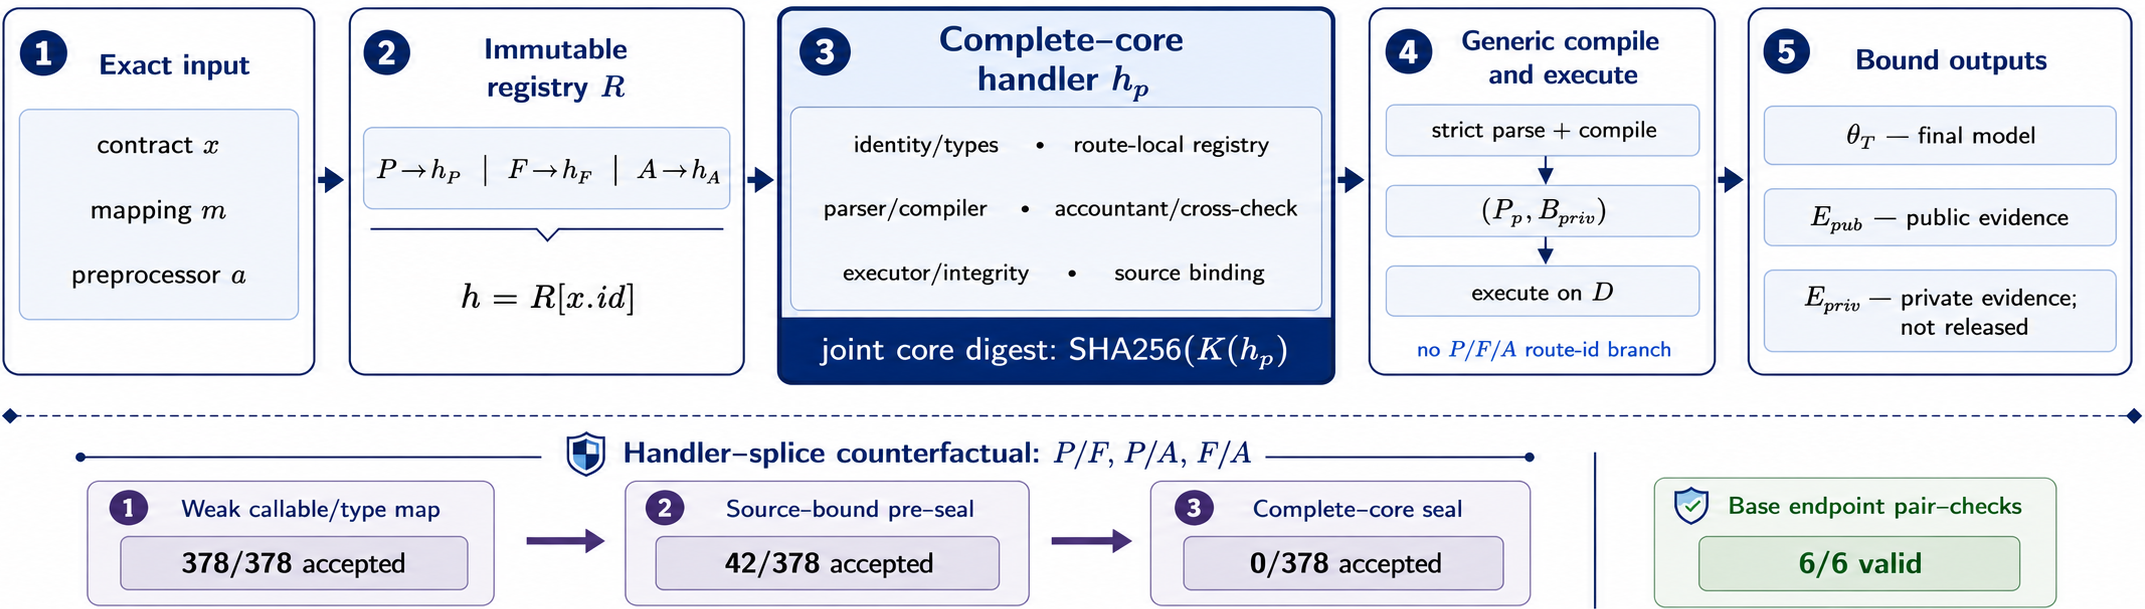
\includegraphics[width=\textwidth]{figures/ch03_source_sealed_compilation.png}
    \caption{Sealed compilation path and handler-splice counterfactual}
    \label{fig:ch3-sealed-compilation}
\end{figure}

Figure~\ref{fig:ch3-sealed-compilation} is the source study's directly extracted
figure asset.  The top lane shows exact input, immutable exact-key selection,
complete-core validation, generic compilation and execution, and separated public
and private evidence outputs.  The lower lane records the nested registration
ablation discussed later.  To preserve the original asset without redrawing it,
the source symbol \(K(h_\rho)\) remains visible in the figure; it denotes the same
complete handler core normalized as \(\RouteCore{h}\) throughout this
dissertation.  No scientific value or label inside the image has been altered.

\subsection{Generic Dispatch, Execution, and Evidence Binding}
\label{subsec:ch3-generic-dispatch}

Let \(\RouteRegistry\) be an immutable map from exact route identifiers to
registered handlers, \(\ContractObject\) an exact serialized contract,
\(m_{\mathrm{map}}\) a generated-record mapping, and \(a_{\mathrm{pre}}\) a fixed
preprocessor.  Generic parsing and compilation form the partial judgment

\begin{equation}
    \RouteRegistry
    \vdash
    \left(
        \ContractObject,
        m_{\mathrm{map}},
        a_{\mathrm{pre}}
    \right)
    \Downarrow
    \left(
        P_{\rho},
        B_{\mathrm{priv}}
    \right).
\label{eq:ch3-compile-judgment}
\end{equation}

The judgment exists only after the following ordered checks.

\begin{enumerate}
    \item Exact-key lookup selects
    \(h=\RouteRegistry[\ContractObject.\mathrm{id}]\), and live registration
    rechecks Equation~\eqref{eq:ch3-registration-judgment}.

    \item The serialized object has the selected handler's exact schema.  The
    dispatcher invokes \(h.p\), then requires the exact returned contract type,
    route identity, and canonical content.  No coercion from a neighboring route
    or fallback parser is allowed.

    \item The dispatcher invokes \(h.c\), requires the exact public-plan type and
    nominal identity, and checks that compilation has not modified the parsed
    contract.

    \item The handler's registered postcompile integrity method reopens the
    public plan, private binding, route profile, mapping and attribution,
    owner-local policy, preprocessor, accountant, executor, and source bundle.
    Every relation must match the selected endpoint.
\end{enumerate}

The generic dispatcher contains no identifier branch for Routes \RouteP, \RouteF,
or \RouteA.  It also has no route-specific contract-type branch or local copy of
route semantics.
Those semantics reside in the selected immutable handler.  The public plan
\(P_{\rho}\) contains the invariant route configuration but omits realized owner
identities, assignments, and sample counts.  The private binding
\(B_{\mathrm{priv}}\) commits to the generated-record mapping, owner attribution,
owner-local policy, and in-memory preprocessor state needed by the executor.

\begin{lemma}[Handler-local conservative extension]
\label{lem:ch3-conservative-extension}
Let
\(\RouteRegistry'=\RouteRegistry\uplus\{j\mapsto h_j\}\), where
\(j\notin\operatorname{dom}(\RouteRegistry)\) and \(h_j\) passes
Equation~\eqref{eq:ch3-registration-judgment}.  If every old handler, its resolved
sources, and its compilation inputs remain unchanged, then any terminating exact
contract whose identifier lies in \(\operatorname{dom}(\RouteRegistry)\) has the
same parse and compilation output under \(\RouteRegistry\) and
\(\RouteRegistry'\).
\end{lemma}

\begin{proof}
Exact-key lookup selects the same immutable old handler in both registries.
Every subsequent parse, compile, and integrity operation is deterministic and
handler-local, and its inputs and resolved sources are unchanged.  The resulting
objects are therefore equal.  The argument is syntactic: it asserts neither
privacy nor semantic correctness of the newly added handler.
\end{proof}

Compilation is followed by a second partial judgment for execution and artifacts:

\begin{equation}
    \left(P_{\rho},B_{\mathrm{priv}}\right);
    \mathcal D
    \Downarrow
    \left(
        \theta_{\TrainingSteps},
        E_{\mathrm{pub}},
        E_{\mathrm{priv}}
    \right).
\label{eq:ch3-execution-judgment}
\end{equation}

This judgment exists only if the compiled object passes its pre-execution check,
the registered route loop completes, the post-execution check passes, and the
output verifier reconstructs every artifact relation.  Here
\(\theta_{\TrainingSteps}\) is the final model parameter vector;
\(E_{\mathrm{pub}}\) contains the public route, accountant results, source
manifest, public metrics, and model serialization; and \(E_{\mathrm{priv}}\)
contains mappings, identities, assignments, and diagnostics that are not
released.

Table~\ref{tab:ch3-lifecycle-evidence} records where each predicate is enforced and
which evidence persists.  Separating these rows is important for the lifecycle
ablation: a strict parser can reject malformed contract fields but cannot detect a
stale private mapping or a public serializer that leaks a private certificate.

\begin{table}[tbp]
    \centering
    \caption{Lifecycle predicates and persisted evidence}
    \label{tab:ch3-lifecycle-evidence}
    \small
    \setlength{\tabcolsep}{3pt}
    \renewcommand{\arraystretch}{1.15}
    \begin{tabular}{@{}
        >{\raggedright\arraybackslash}p{0.18\textwidth}
        >{\raggedright\arraybackslash}p{0.24\textwidth}
        >{\raggedright\arraybackslash}p{0.48\textwidth}@{}}
        \toprule
        \textbf{Boundary} &
        \textbf{Enforced at} &
        \textbf{Persisted evidence} \\
        \midrule
        Registration &
        Registry &
        Core, report, and seven source witnesses \\

        Contract &
        Parser/compiler &
        Route, contract, and profile digests \\

        Data &
        Compiler/executor &
        Private mapping, policy, and transform bindings \\

        Accounting &
        Compiler/verifier &
        Two values and theorem/configuration identity \\

        Loop &
        Executor/tests &
        Declarations, diagnostics, and reference replay \\

        Links &
        Serializer/verifier &
        Model, execution, bundle, summary, and collection \\
        \bottomrule
    \end{tabular}
\end{table}

Structured contracts are loaded with duplicate-key detection, exact primitive and
nominal types, and rejection of extra fields.  Dataset contracts must equal a
versioned benchmark profile for every profile-controlled value.  Compilation
checks contiguous unique row indices, unique generated-record identifiers,
nonempty labels, exactly one owner per record, and a full mapping digest.  The
wrapper binds transformed features, labels, mapping, policy, and preprocessor
before compilation and at every execution.  The fixed affine preprocessor checks
dimensions and finite scales, declares that it has not been fitted on protected
data, and is applied inside the executor rather than replaced by caller-supplied
features.

The two accounting values in
Table~\ref{tab:ch3-lifecycle-evidence} are route-internal cross-checks, not two
independent privacy theorems.  Route \RouteP{} recomputes fixed-order RDP through
separately exposed compatible implementations and claims arithmetic
correspondence, not executor equivalence.  Route \RouteF{} compares a library
calculation with a direct fixed-size computation using normalized noise
\(\sigma/2\).  Route \RouteA{} compares its floating-point conservative
random-allocation calculation with a separately structured high-precision
implementation.  Numerical agreement can expose implementation drift, but both
paths could still share a mistaken theorem premise.

Artifact verification preserves both sides of the public/private boundary.
Public serialization contains fixed route and accountant declarations, the source
manifest, public-benchmark metrics, and an exact float32 non-pickle model.
Realized owner identities, random-allocation assignments, mapping commitments,
sample counts, and diagnostic traces remain private.  Model, execution, bundle,
summary, and collection identifiers are linked so that a valid number cannot be
detached from the plan and model to which it belongs.

\subsection{Conditional Privacy Scope}
\label{subsec:ch3-conditional-scope}

The registration judgment supports a route-conditional privacy statement, not an
unconditional certificate.  Consider a release procedure that is total over its
declared adjacent domain; completes a fixed schedule without a data-dependent
abort; keeps validation and diagnostic outputs internal; fixes preprocessing and
the owner-local contribution rule independently of protected input; contributes
at most one vector of norm \(C\) for each participating owner; and adds independent
Gaussian noise at every scheduled step.  If the procedure then uses

\begin{itemize}
    \item Route \RouteP{} with its registered Bernoulli/add-remove accountant,
    \item Route \RouteF{} with its registered fixed-size/replace-one bound and
    sensitivity \(2C\), or
    \item Route \RouteA{} with its registered per-epoch uniform
    \(\AllocationCount\)-of-\(t\) allocation/add-remove bound,
\end{itemize}

the applicable prior analysis yields owner-level
\((\varepsilon,\delta)\)-DP for the final model under the declared
adjacency~\cite{wang2019subsampled,birrell2024fixed,
shenfeld2025randomallocation,dong2026optimal}.  Fixed division, optimizer updates,
and final-model release are post-processing.  This statement restates established
premises.  Evidence-sealed registration records and cross-checks the declared
objects, but it does not prove that arbitrary executor code satisfies them.

Four domain-separated pseudorandom streams cover initialization, owner sampling,
within-owner selection, and Gaussian noise in the research implementation.  The
frozen backend uses NumPy PCG64 for reproducibility and records
\path{secure_rng=false}.  This is an explicit nondeployment setting.  Random coins,
owner identities, mappings, and realized sample statistics remain private, but
keeping them private does not make the generator cryptographically secure.

The checked threat model targets accidental drift, stale results, ordinary
misconfiguration, and substitutions visible in declared inputs, source, or
outputs.  It assumes SHA-256 collision resistance and honest source, executor,
evidence builder, and verifier.  A malicious component could fabricate matching
hashes, select weak noise while writing a stronger declaration, or exfiltrate
private diagnostics.  Exceptions and rejection messages can themselves leak
input-dependent behavior and therefore are local controls rather than DP outputs.
Timing, hardware, operating-system, and other side channels are outside scope.

The benchmark compilers further require exact public-fixture mappings and can
reject changed inputs.  They are not total private-domain release algorithms, so
every reported execution is labeled \path{research_non_release}; its accountant
value is an integration result rather than a deployment claim.  Deployment would
require audited secure randomness, data-independent and total failure behavior,
validated composition across releases, and stronger provenance or execution
evidence.  Hash equality cannot establish hidden random coins, and a single-owner
route analysis cannot be extended to multi-owner records without a new adjacency
and sensitivity argument.

\section{Experimental Evaluation}
\label{sec:ch3-evaluation}

The evaluation asks four bounded questions.

\begin{enumerate}
    \item[\textbf{Q1.}] Do lifecycle bindings reject fixed failures that remain
    after strong contract-only parsing?

    \item[\textbf{Q2.}] Does the complete-core seal reject handler splices that
    pass simpler registration checks?

    \item[\textbf{Q3.}] Can the registry add a structurally different route without
    changing old outputs, while separating controlled route and contract surfaces?

    \item[\textbf{Q4.}] Do route-specific accountants, executors, and artifact
    checks correspond to the registered endpoints on the fixed integration grid?
\end{enumerate}

These are bounded conformance questions.  A count is exhaustive only within its
named, prespecified finite universe.  The deterministic fractions do not estimate
defect prevalence, held-out recall, or population error.  Likewise, the fixed-seed
executions test compiler, executor, and artifact correspondence; they do not
compare utility among mechanisms with different adjacencies and calibration.

\subsection{Lifecycle and Handler-Splice Ablations}
\label{subsec:ch3-lifecycle-ablation}

\paragraph{Protocol and research profiles.}
The integration grid uses the UCI Human Activity Recognition (HAR) dataset
~\cite{anguita2013har,reyesortiz2013uci}, the WISDM
activity-recognition dataset~\cite{kwapisz2011activity}, and the PhysioNet 2019
sepsis data~\cite{reyna2019sepsis,reyna2020sepsis,goldberger2000physiobank}.
Their public owner-disjoint protocols contain, respectively, \(21/9\), \(25/11\),
and \(312/78\) nominal train/test owners.  The corresponding generated-record
counts are \(7{,}352/2{,}947\), \(7{,}049/3{,}331\), and
\(1{,}601/398\).  Registered affine transforms produce 561, 24, and 240 features.
Each dataset--route profile uses a linear classifier and five fixed seeds.

All nine profiles target
\((\varepsilon,\delta)=(8,10^{-5})\).
Table~\ref{tab:ch3-route-profiles} reproduces the exact public route values.
Every displayed Route \RouteA{} profile has one epoch, so
\(\TrainingSteps=t\).  Route \RouteF{} uses replace-one sensitivity \(2C\);
Routes \RouteP{} and \RouteA{} use add/remove sensitivity \(C\).  The table is a
registration fixture, not a claim that the three route laws are equivalent or
that their calibrated utility is directly comparable.

\begin{table}[tbp]
    \centering
    \caption{Registered owner-sampled DP-SGD research profiles}
    \label{tab:ch3-route-profiles}
    \scriptsize
    \setlength{\tabcolsep}{1.7pt}
    \renewcommand{\arraystretch}{1.13}
    \begin{tabular}{@{}
        >{\raggedright\arraybackslash}p{0.13\textwidth}
        c
        >{\raggedright\arraybackslash}p{0.39\textwidth}
        c
        >{\centering\arraybackslash}p{0.10\textwidth}
        r
        c@{}}
        \toprule
        \textbf{Dataset} &
        \textbf{Route} &
        \textbf{Adjacency / participation law} &
        \(\boldsymbol{\TrainingSteps}\) &
        \textbf{\(k\) or \(m\)} &
        \(\boldsymbol{\sigma}\) &
        \(\boldsymbol{D_{\mathrm{norm}}}\) \\
        \midrule
        UCI HAR & \RouteP &
        add/remove; Bernoulli \(\SamplingRate=0.380952\) &
        15 & -- & 1.269710 & 8 \\
        UCI HAR & \RouteF &
        replace-one; SRSWOR \(m/\OwnerPopulation=8/21\) &
        15 & \(m=8\) & 3.806632 & 8 \\
        UCI HAR & \RouteA &
        add/remove; uniform \(k\)-of-\(T\) allocation &
        15 & \(k=6\) & 1.229575 & 8 \\
        \addlinespace
        WISDM & \RouteP &
        add/remove; Bernoulli \(\SamplingRate=0.320000\) &
        20 & -- & 1.251026 & 8 \\
        WISDM & \RouteF &
        replace-one; SRSWOR \(m/\OwnerPopulation=8/25\) &
        20 & \(m=8\) & 3.838696 & 8 \\
        WISDM & \RouteA &
        add/remove; uniform \(k\)-of-\(T\) allocation &
        20 & \(k=6\) & 1.090646 & 8 \\
        \addlinespace
        Sepsis & \RouteP &
        add/remove; Bernoulli \(\SamplingRate=0.100000\) &
        50 & -- & 0.857344 & 32 \\
        Sepsis & \RouteF &
        replace-one; SRSWOR \(m/\OwnerPopulation=32/312\) &
        50 & \(m=32\) & 2.380381 & 32 \\
        Sepsis & \RouteA &
        add/remove; uniform \(k\)-of-\(T\) allocation &
        50 & \(k=5\) & 0.776173 & 32 \\
        \bottomrule
    \end{tabular}
\end{table}

\paragraph{Q1: lifecycle.}
The first boundary loads a contract with duplicate-key detection and then
invokes the selected route's exact parser.  It excludes mapping and preprocessor
compilation, backend approval, data/execution binding, compiled-object integrity,
and public artifact redaction.  The frozen Route \RouteP{} lineage contains 52
targeted mutations and eight reproduced historical failures fixed before stage
attribution.  Each case is assigned to its earliest rejecting boundary.

The strong contract-only boundary rejects \(36/52\) targeted mutations and
\(5/8\) historical cases.  For the targeted set, mapping and preprocessor
compilation adds ten rejections, backend approval adds one, and compiled integrity
adds five, bringing the full lifecycle to \(52/52\).  For the historical set,
exact data/execution binding catches two stale mappings and the public-artifact
boundary catches one certificate containing information that should have remained
private, bringing the full lifecycle to \(8/8\).

This result isolates the role of downstream bindings.  The additional 16 targeted
and three historical rejections are not evidence that strict parsing was weak; the
cases were constructed precisely so that their earliest observable inconsistency
could occur after parsing.  Nor do the ratios measure detection performance on
future defects.  The historical cases were retrospectively selected and the
targeted set is an authored control corpus, not a random or held-out sample.

\paragraph{Q2: discriminating registration ablation.}
The handler experiment partitions each endpoint into seven prespecified binary
surfaces: identity and report; contract and plan types; parser; compiler;
route-local registry; accountant and cross-check; and executor, integrity, and
source binding.  For each of the pairs \RouteP/\RouteF, \RouteP/\RouteA, and
\RouteF/\RouteA, the two unmodified endpoints are excluded, leaving
\(2^7-2=126\) distinct nonendpoint splices.  The declared universe therefore
contains

\begin{equation}
    3\left(2^7-2\right)=378
\label{eq:ch3-handler-lattice}
\end{equation}

hybrids.

The weak boundary checks only a generic callable/type map and accepts
\(378/378\).  A source-bound pre-seal additionally checks nominal fields,
obligations, callable resolution, and source digests, but has no passing report
committed to the complete core; it accepts \(42/378\), exactly 14 in each route
pair.  Those survivors can splice a coherent parser, compiler, or
accountant/cross-check block while keeping individually valid source witnesses.
The complete-core predicate in
Equation~\eqref{eq:ch3-registration-judgment} accepts \(0/378\) hybrids, while all
six unmodified endpoint checks across the three pairs pass.  These are the
378/42/0 results shown in Figure~\ref{fig:ch3-sealed-compilation}.

A separate verifier that does not import the report builder reconstructs every
combination and decision.  Eight additional registration mutations---including a
missing or duplicate obligation, changed source or report digest, spliced
parser/type, unvalidated executor, and duplicate route---also fail.  The conclusion
is exact only for the authored lattice: every prespecified nonendpoint splice is
prevented from retaining either endpoint label.  Rejection neither establishes a
privacy violation nor covers unmodeled fields or arbitrary third-party handlers.

\subsection{Route Separation, Extension, and Verification}
\label{subsec:ch3-extension-verification}

\paragraph{Q3: matched-shell separation.}
The first separation control holds the scientific configuration fixed rather than
simply counting distinct implementations.  Within each \RouteP/\RouteF{} dataset
pair, 38 fields are exact matches, including the dataset and split, privacy target,
schedule, clipping threshold, contribution cap, model, optimizer, loss, and fixed
preprocessor.  Eight prespecified obligation families---route, schema, adjacency,
sampler, accountant/theorem, executor, noise, and the complete
mechanism/accountant surface---are substituted in both directions over the three
datasets.

All \(48/48\) nonvacuous substitutions fail: 12 at exact-key dispatch and 36 at
the selected route's strict contract.  Thus the two endpoints remain distinguishable
when 38/38 surrounding fields are held fixed.  The causal statement is limited to
those 48 authored substitutions; it is not semantic completeness for every
possible route difference.

\paragraph{Branch-free extension.}
Source inspection confirms that the generic parser/compiler contains none of the
three route identifiers or contract types and no conditional branch of the form
\path{if route_id == ...}.  All nine dataset--route contracts compile.  Adding
Route \RouteA{} to the \RouteP/\RouteF{} registry leaves the six old parsed
contracts and public plans structurally equal and preserves their exact digests,
including equality to frozen predecessor outputs.  This is the empirical instance
of Lemma~\ref{lem:ch3-conservative-extension}.

As a separate extension stress test, an external handler \(\mathsf H\) overlays a
privately maintained privacy-loss-distribution accountant on Route \RouteA's
unchanged mechanism and executor.  All four relevant handler endpoints validate,
all nine old \RouteP/\RouteF/\RouteA{} contract--plan outputs remain byte-exact,
and the complete core rejects \(756/756\) nonendpoint handler hybrids across six
pairs.  This establishes bounded preservation for one external accountant overlay;
it is not a fourth mechanism and does not establish arbitrary plugin support.

At the serialized-contract layer, each pair is separately partitioned into eight
disjoint surfaces: identity, execution, privacy/accounting, data lineage, schedule,
noise geometry, update contribution, and optimizer/sampler.  Across three route
pairs and three datasets, both endpoints parse and all

\begin{equation}
    9\left(2^8-2\right)=2{,}286
\label{eq:ch3-contract-lattice}
\end{equation}

nonendpoints fail.  Strict route parsers explain much of this second lattice, so
the result supports route separation rather than the central complete-core
novelty.  It complements, but does not replace, the handler-level 378/42/0
counterfactual.

\paragraph{Q4: accountant and execution correspondence.}
For Route \RouteA, the production direct calculation and the separately structured
high-precision implementation agree for all three profiles, both add/remove
privacy directions, and every registered order.  Six mutations to the bound
accountant-query identity and 13 invalid inputs are exercised.  External
privacy-loss-distribution values in the frozen gate are nonauthorizing
comparisons; only the separately registered \(\mathsf H\) handler can make its own
route-conditional statement.

An independent reference executor that imports no production execution
implementation matches \(15/15\) Route \RouteA{} runs, \(425/425\) scheduled
steps, \(9{,}180/9{,}180\) owner vectors, and \(30/30\) final model tensors.  A
separate fixture contains a true empty step and confirms that Gaussian noise is
generated for both model tensors and that the optimizer advances.  Routes
\RouteP{} and \RouteF{} retain \(30/30\) exact run replays, covering \(850/850\)
steps and \(60/60\) final tensors.  The Route \RouteA{} public archive also
rebuilds deterministically and contains no checked private assignment or identity
field.

Together, the 15 Route \RouteA{} and 30 \RouteP/\RouteF{} runs form a
\(45/45\) fixed-seed integration grid.  Different adjacency definitions and
noise calibration make this grid unsuitable for utility or inferential comparison.
Its evidential role is exact correspondence among registered plans, accountants,
executor traces, reference replays, and serialized artifacts.

Table~\ref{tab:ch3-evidence-authority} binds every reported result to its artifact,
verifier, and exact denominator.  The row structure also prevents a count from
being cited without the boundary that gives it meaning.

\begin{table}[tbp]
    \centering
    \caption{Evidence artifacts, verifiers, and exact denominators}
    \label{tab:ch3-evidence-authority}
    \footnotesize
    \setlength{\tabcolsep}{2.2pt}
    \renewcommand{\arraystretch}{1.13}
    \begin{tabular}{@{}
        >{\raggedright\arraybackslash}p{0.40\textwidth}
        >{\raggedright\arraybackslash}p{0.26\textwidth}
        >{\raggedright\arraybackslash}p{0.24\textwidth}@{}}
        \toprule
        \textbf{Evidence role and bound artifact} &
        \textbf{Verifier or comparator} &
        \textbf{Exact result} \\
        \midrule
        Endpoint conformance; route reports &
        Registration verifier &
        \(3/3\); \(7/7\) per handler \\

        Lifecycle attribution; frozen \RouteP{} manifests &
        Stage verifier &
        \(36/52\) vs.\ \(52/52\);
        \(5/8\) vs.\ \(8/8\) \\

        Matched-shell ablation; \RouteP/\RouteF{} substitution report &
        Separate verifier &
        \(48/48\); \(38/38\) fixed \\

        Compilation/extension; contracts and plans;
        \newline frozen \RouteP, \RouteF, and \(\mathsf H\) outputs &
        Compiler/digest verifiers &
        \(9/9\); \(6/6\);
        \(\mathsf H\) \(4/4,\ 9/9\) \\

        Finite-lattice conformance; three-, six-, and nine-pair reports &
        Separate verifier &
        \(378/378\); \(756/756\);
        \(2{,}286/2{,}286\) \\

        \RouteA{} integration; trace bundle and empty-step fixture &
        Reference executor/comparator &
        \(15/15\); \(425/425\);
        \(9{,}180/9{,}180\);
        \(30/30\); \(1/1\) \\

        \RouteP/\RouteF{} integration; trace bundles &
        Reference executor &
        \(30/30\); \(850/850\);
        \(60/60\) \\

        Focused/full regression conformance; logs &
        Test runner &
        \(44/44\); \(154/154\) run;
        \(7/161\) skip \\
        \bottomrule
    \end{tabular}
\end{table}

Reproducibility controls reject duplicate serialization keys and recompute table
aggregates.  Separate verifiers reclassify the 60 contract-only lifecycle cases
and reconstruct the 48 matched-shell substitutions, handler and contract lattices,
conservative-extension rows, route reports, private diagnostics, source links, and
registered traces.  Focused route-accounting, compilation, execution,
registration, and lattice tests pass \(44/44\).  The full frozen regression
collects 161 tests: all \(154/154\) executed tests pass and seven raw-data-scoped
cases skip.  The skips are reported rather than included in the executed-test
denominator.

The evidence authority remains finite and honest-source.  Lifecycle counts are
retrospective stage attribution; the handler and contract lattices are exhaustive
only over their declared binary surfaces; the matched shell contains 48
prespecified substitutions; and the integration grid contains fixed seeds rather
than a sample of deployment outcomes.  Deterministic full-universe predicates
within those sets have no sampling error, so a significance test would not add a
meaningful population interpretation.  None of the results in
Table~\ref{tab:ch3-evidence-authority} proves privacy, arbitrary-input refinement,
or adversarial execution attestation.

\clearpage
\section{Synthesis of Auditable Privacy}
\label{sec:ch3-auditable-privacy-synthesis}

The two chapters in the \AuditablePrivacy{} axis intervene at different times.
Chapter~\ref{ch:post-execution-validation} begins with a completed execution and a
frozen evidence bundle.  It determines whether that evidence licenses a direct,
converted, grouped, or blocked privacy-unit sentence.  The present chapter begins
with an exact contract before training.  It prevents an installed mixture of
adjacency, sampler, sensitivity, accountant, executor, transformation, and
evidence obligations from retaining an existing route label.

The relationship is diagnosis followed by prevention, but neither mechanism
subsumes the other.  Post-execution evidence validation can expose unsupported
wording even when no pre-execution registry was used, yet it cannot repair an
already executed route.  Evidence-sealed registration can reject a mixed route
before dispatch, yet it does not decide every public sentence that a later frozen
execution may support.  It also does not authenticate that the reported execution
occurred.  Together, the chapters narrow the gap from both sides without claiming
end-to-end DP certification.

Four common design principles emerge.  First, \emph{claim specification} fixes the
unit, adjacency, route identity, and numerical target before a positive statement
is interpreted.  Second, \emph{mechanism binding} connects that specification to
the actual sampler, contribution geometry, accountant, executor, transformation,
and schedule.  Third, an \emph{evidence-bound decision} requires the relevant
mapping, source, runtime, and artifact relations rather than inferring assurance
from an isolated number or label.  Fourth, \emph{fail-closed behavior} blocks the
positive interpretation when a required relation is missing or inconsistent.

This is the privacy-side instantiation of \ClaimAlignedAssurance{}.  The
contribution is not a claim that every registered system is trustworthy.  It is a
disciplined rule for determining when a particular privacy claim remains aligned
with its protected object, installed mechanism, and observable evidence, together
with explicit boundaries where that determination stops.  The next chapter moves
to the second dissertation axis, \SecurePublicVerification{}, where the assurance
object changes from a privacy statement about training to independently
verifiable provenance for generative-AI content.
